%!TEX root = ../../report.tex

\subsection{Modern OpenGL} % (fold)
\label{sub:modern_opengl}

Majors changes has been imposed to this library from it's early versions and this section covers the modern version of OpenGL, after version 3.2.

OpenGL is an well known cross-platform Application Programming Interface (API) created by Silicon Graphics Computer Systems with Version 1.0 released in July of 1994 for 3-D Graphics and Imaging. It's a streamlined and hardware-independent interface that can be implemented on many different types of graphics hardware. It's also independent of the machine's operative and windowing systems.

OpenGL provides a small set of geometric primitives - points, lines, triangles and patches that are specified by their vertices. And from this geometric primitives all geometry is constructed, both in 2D and 3D. 

Shaders ``are special functions that the graphics hardware executes. The best way to think of shaders is as little programs that are specifically compiled for your graphics processing unit''. \cite{shreiner2013opengl}

There are some steps that are performed to render an image. First the model is created from geometric primitives and this data is the input  for the pipeline(Vertex Data) in Figure~\ref{fig:OGLPipeline}. 

\begin{figure}[htbp]
	\centering
	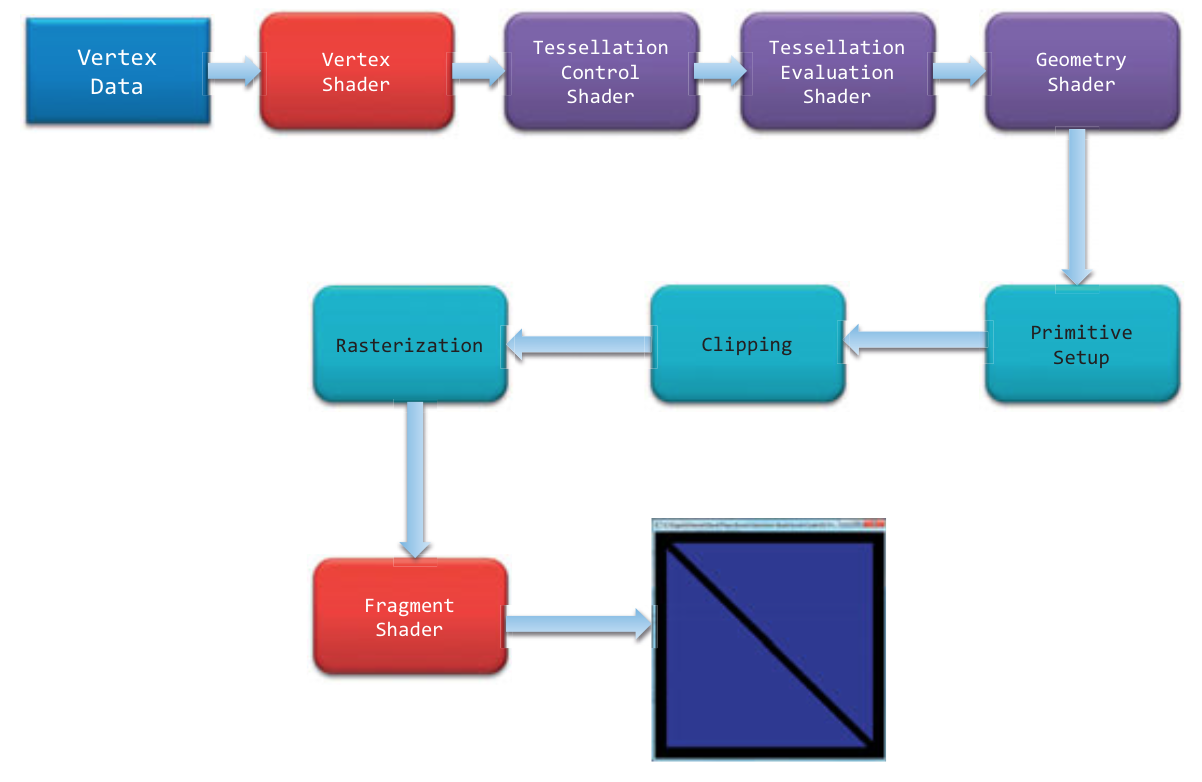
\includegraphics[width=0.95\textwidth]{img/OpenGL/pipeline.png}
	\caption{OpenGL Pipeline \cite{shreiner2013opengl}}
	\label{fig:OGLPipeline}
\end{figure}


The first step of the pipeline is the Vertex Shader that process the data associated with each vertex. 

After this, there are three optional shaders. In this three there are two Tessellation Shaders. With this shaders simple geometries can be tessellated and increase of the number of primitives to improve the models dynamically.

The third optional shader is the Geometric Shader that allows the additional processing of geometric primitives and also including the creation of new primitives.

Until now all steps work with vertices, and after those steps there are three fixed steps, primitive assembly, clipping and rasterization that assembly the vertices into primitives, clip the geometry cutting the parts that falls of the ``screen'' and the generation of fragments respectively.

A fragments is a ``‘candidate pixel’, in that pixels have a home in the framebuffer, while a fragment still can be rejected and never update its associated pixel location'' \cite{shreiner2013opengl}.
\subsection{Vertex Shaders} % (fold)
\label{sub:vertex_shaders}
Vertex Shaders can be very simple, from a \emph{pass-through shader} that just copies the data to the next step to very complex ones.

In this shaders are used to performed computations to calculate the position of the vertices in screen coordinates, assign vertex's color using lightning computations, etc..

Vertex Shaders have some limitations, they cannot create additional geometry and cannot access data of other vertices. They can just process the data of the current vertex and the number of vertices after this step is the same as before.

% subsection vertex_shaders (end)

\subsection{Tessellation Shaders} % (fold)
\label{sub:tesselation_shaders}
Tessellation Shaders are very different form the previous ones. This shaders address some of limitations presented before.
This shaders work with a geometric primitive called a \emph{patch}. A patch is a list of vertices that preserves their order during processing. This is because each patch can have an arbitrary number of vertices that have to be specified before drawing opposing to the other primitives that have a specific/pre-assigned/fixed number of vertices.

\subsubsection{Tessellation Control Shader} % (fold)
\label{ssub:tesselation_control_shader}
	This shader defines the layout of the output through the generation of the tessellation output-patch vertices and the specification of the tessellation level factors. The output-patch vertices is the list of vertices that results after the input vertices have been processed. The tessellation level factor defines how much the output patch is tessellated. 

	OpenGL supports three tessellation domains: a quadrilateral, a triangle, and a collection of isolines \cite{shreiner2013opengl}. To control the amount of tessellation two sets of values are set, the outer-tessellation values and the inner-tessellation values. This values define how the perimeter or the interior of the domain are subdivided respectively. 

% subsubsection tesselation_control_shader (end)

\subsubsection{Tessellation Evaluation Shaders} % (fold)
\label{ssub:tesselation_evaluation_shaders}
Tessellation shaders work with the output of the previous phase. Here the vertex positions are calculated from the tessellation computed before. It's is basically responsible for the calculation of the vertices screen positions from the layout defined.

% subsubsection tesselation_evaluation_shaders (end)

% subsection tesselation_shaders (end)

\subsection{Geometry Shaders} % (fold)
\label{sub:geometriy_shaders}

Geometry Shaders are the first shaders that access the complete primitive as a list of vertices and with that it's allowed to do different actions that require this access to information. The amount of output can be variable so both \emph{culling geometry} and \emph{geometry amplification}, respectively output less vertices that the input and output more vertices than the input. Also in this shaders the primitives type can be modified, i. e. the input can be \emph{quads} and the output be a \emph{triangle\_strip}.

Geometry shaders however have a limitation. Each call of a geometry shader have a maximum number of vertices that it can output. This limitation could be important for the implementation of geometry amplification. This maximum number is hardware dependent and varies with the size of the output buffer that is used by the GPU to support geometry shaders.

% subsection geometriy_shaders (end)

\subsection{Fragment Shaders} % (fold)
\label{sub:fragment_shaders}
This shaders implement the last phase of the pipeline. Here the fragment's final color is computed and also the depth value.

Fragment Shaders are useful to implement texture mapping or lights for instance.

% subsection fragment_shaders (end)
% subsection modern_opengl (end)